\documentclass[a4paper,12pt]{article}
\setlength{\parskip}{1em} % 調整段落間距為 1em

% 設定頁面邊界
\usepackage[margin=2cm]{geometry}

% 字體設定
\usepackage{fontspec} % 設定字體
\usepackage{xeCJK} % 讓中英文字體分開設置
\setmainfont[
    BoldFont={Times New Roman Bold},
    ItalicFont={Times New Roman Italic}
]{Times New Roman}
\setCJKmainfont[
    BoldFont={標楷體},
    ItalicFont={標楷體} % 標楷體沒有斜體,可以重複設置
]{標楷體}
\XeTeXlinebreaklocale "zh" % 中文自動換行
\XeTeXlinebreakskip = 0pt plus 1pt

% 其他套件
\usepackage{graphicx} % 插入圖片
\usepackage{indentfirst} % 首行縮排
\usepackage{titlesec} % 調整標題格式
\usepackage{hyperref} % 超連結
\usepackage{cite} % 引用管理

% 調整章節標題格式
\titleformat{\section}
  {\normalfont\Large\bfseries}{\thesection}{1em}{}
\titleformat{\subsection}
  {\normalfont\large\bfseries}{\thesubsection}{1em}{}

% 開始文件
\begin{document}

% 封面
\begin{titlepage}
  \begin{center}
    \vspace*{2cm}
    {\fontsize{16pt}{16pt}\selectfont 國立臺灣師範大學 資訊工程學系}\\[1cm]
    {\fontsize{16pt}{16pt}\selectfont 113 資訊專題研究(一)期末書面報告}\\[4cm]
    {\fontsize{16pt}{16pt}\selectfont 釣魚攻擊與防禦的紅藍對抗實踐}\\[1cm]
    {\fontsize{16pt}{16pt}\selectfont Phishing Attack and Defense: A Practical Red-Blue Team Exercise}\\[9cm]
    {\fontsize{12pt}{12pt}\selectfont 指導教授 官振傑 教授}\\[0.5cm]
    {\fontsize{12pt}{12pt}\selectfont 學生 李曜宇 撰}\\[0.5cm]
    {\fontsize{12pt}{12pt}\selectfont 中華民國 113 年 12 月}
  \end{center}
\end{titlepage}

\newpage

% 摘要
\section{摘要}
當代網路安全領域中,釣魚攻擊依然是最常見且最具成效的入侵手段之一。尤其在高階持續性威脅(Advanced Persistent Threat, APT)攻擊中,攻擊者通常透過精心設計的釣魚郵件或釣魚網站,引誘目標用戶點擊惡意連結或下載惡意附件,從而獲取系統的初始訪問權限。本專題旨在深入探討釣魚攻擊的技術與策略,並提出有效的防禦對策。

為了更全面地理解釣魚攻擊的實際流程與手法,我們在本學期內,在合法合規的前提下,以國立臺灣師範大學的 Moodle 系統作為模擬目標,實際製作了一個釣魚網站。這一過程讓我們能夠更加直觀地掌握釣魚攻擊的實施步驟及其技術細節,為後續的防禦策略設計提供了寶貴的實踐經驗。

% 研究動機與研究問題
\section{研究動機}
隨著網路技術的迅速發展,企業和組織在享受數位化帶來便利與效率的同時,也面臨前所未有的網路安全挑戰。特別是在數位經濟持續擴張的背景下,敏感資料的保護、業務運行的穩定性以及資訊系統的完整性,已成為企業核心運營中不可或缺的基石。然而,網路安全威脅的形式不斷演變,其中以高階持續性威脅(Advanced Persistent Threat, APT)攻擊最為棘手,已成為現代企業面臨的重大挑戰之一。

APT 攻擊不同於傳統攻擊,其特點在於高度的針對性與隱蔽性。攻擊者常將釣魚郵件作為進攻的首要手段,結合技術漏洞與社交工程,藉此以相對低的成本實現高效的系統入侵。一封看似普通的郵件可能隱藏著精心設計的惡意鏈接或附件,受害者在無意間點擊後,便可能讓攻擊者成功滲透內部系統。這類攻擊往往具有極高的成功率,且隱蔽性強,即使企業部署了基礎安全措施,也可能難以防範。

為了避免對釣魚攻擊的理解僅停留在概念層面,我們選擇採取雙向學習的方式,從實踐中獲得對攻擊與防禦的全面認識。首先,我們從紅方(攻擊者)的視角出發,親身模擬並實踐釣魚攻擊的完整流程,剖析攻擊者的行動邏輯與技術實現。這樣的實踐不僅幫助我們深入理解攻擊者的思維模式與技術細節,也為設計針對性的防禦策略提供了實踐依據。此外,我們預計之後會站在藍方(防禦者)的立場,設計和實施有效的防禦措施,包括提升人員對釣魚攻擊的防範意識,以及構建技術層面的釣魚攻擊偵測與阻斷機制。

透過這種紅藍對抗的雙重角色轉換,我們期望模擬真實的攻擊與防禦場景,建立一個完整的對抗演練環境,以驗證釣魚攻擊與防禦策略的實際效能。我們希望,這一研究能為網路安全領域提供實用建議,幫助更多企業應對新型威脅,進一步促進整體安全生態的健康發展。

% 研究問題
\section{研究問題}
本專題欲研究之問題如下:
\begin{enumerate}
  \item 如何構建一個紅藍對抗環境來驗證攻防策略的效能?
  \item 如何有效地設計和實施釣魚攻擊,突破目標的安全防線?
  \item 紅方在成功釣魚後會採取哪些後續行動?
  \item 如何開發有效的防禦措施來預防和偵測釣魚攻擊?
  \item 如何設計防禦措施以應對紅方的進一步行動?
\end{enumerate}

% 文獻回顧與探討
\section{文獻回顧與探討}

\subsection{APT 的定義}

進階持續性威脅(Advanced Persistent Threat, APT)是一種高度針對性且隱蔽的網路攻擊,通常由具備高超專業技能與豐富資源的攻擊者發起。我們採用了美國國家標準與技術研究院(NIST)對 APT 的定義:「APT 是一個具備高超專業技能和豐富資源的對手,能夠利用多種攻擊向量(如網絡、實體和欺騙手段)創造機會來達成其目標。這些目標通常包括在目標組織的信息技術基礎設施中建立並擴大立足點,目的是竊取信息、破壞或妨礙某些關鍵任務、計畫或組織,或者準備將來實施這些目標。進階持續性威脅具備以下特徵:(i)在長期內反覆追求其目標;(ii)適應防禦者抵抗它的努力;(iii)決心維持實現其目標所需的交互。」

NIST 的定義清晰地闡明了 APT 的核心特徵,基於此定義,我們總結了 APT 的以下顯著特徵:

\begin{itemize}
    \item 具體目標與明確目的:APT 攻擊通常針對特定的目標,這些目標多為擁有大量知識產權的政府機構或企業。攻擊行動具有明確的戰略目的,例如獲取情報或破壞關鍵基礎設施。
    \item 高超技能與資源支持:APT 攻擊者往往是一群高度組織化的專業黑客團隊,可能隸屬於國家支持的網絡部隊,或被僱傭為網絡僱傭兵。他們擁有豐富的資源,能長期支持攻擊行動,並開發或購買零日漏洞及其他攻擊工具。
    \item 隱蔽性與持續性:APT 攻擊者能在目標系統中潛伏數月甚至數年。他們採用低調行動以避免被檢測,並根據目標的防禦策略動態調整攻擊技術。
\end{itemize}

APT 的這些特徵使其成為現代網路安全領域中最具挑戰性的威脅之一,也突顯了研究針對 APT 攻擊之防禦策略的重要性。

\subsection{APT 攻擊的階段}

APT 攻擊是一種高度精密且持續的網路攻擊,其運作通常分為六個階段。這些階段基於「入侵殺傷鏈」(intrusion kill chain)的模型,有助於理解攻擊者的行動方式,並為防禦策略的設計提供指導。

\begin{enumerate}
    \item \textbf{偵查與武器化}:
    APT 攻擊的第一步是偵查目標組織,收集其技術環境與關鍵人員的相關信息。攻擊者通常利用社交工程和開源情報(OSINT)工具進行情報收集:
    \begin{itemize}
        \item \textbf{社交工程}:心理操縱受害者執行特定操作,例如點擊惡意鏈接或提供敏感信息。
        \item \textbf{開源情報(OSINT)}:通過公開網絡資源獲取數據,並使用數據挖掘技術生成可行的攻擊計劃。
    \end{itemize}

    \item \textbf{傳遞}:
    攻擊者將攻擊載具(如惡意代碼)傳遞給目標。常見的方法包括:
    \begin{itemize}
        \item \textbf{針對性釣魚攻擊(Spear Phishing)}:根據偵查階段的信息,設計個性化的釣魚郵件,誘導目標下載惡意附件或點擊惡意鏈接。
        \item \textbf{水坑攻擊(Watering Hole Attack)}:攻擊者感染目標經常訪問的合法網站,使訪問者無意中執行惡意代碼。
    \end{itemize}

    \item \textbf{初始入侵}:
    攻擊者利用漏洞實現初始入侵,獲得未經授權的訪問權限。他們通常會安裝後門軟件,建立長期立足點,為後續攻擊活動創造條件。

    \item \textbf{指揮與控制(C2)}:
    攻擊者利用指揮與控制機制遠程操控受感染設備,並隱蔽通信,進一步實施攻擊。他們可能使用:

    \item \textbf{橫向移動}:
    攻擊者在網絡內部橫向移動,尋找更多目標系統,並提升訪問權限。他們通常進行內部偵查、入侵其他系統以獲取數據,並維持對網絡的長期控制。

    \item \textbf{數據竊取}:
    最終,攻擊者會壓縮、加密並傳輸數據到其控制的外部服務器。他們通常利用 SSL/TLS 協議或匿名網絡來隱藏數據傳輸過程,避免被防禦系統檢測。\cite{2014aptstudy}
\end{enumerate}


\subsection{APT初始入侵之實務}
我們回顧了伊朗APT組織在多起攻擊中所使用的初始入侵之手法,圖一顯示了針對十一個伊朗背景的行動群組分析,他們使用多種向量進行初始攻擊,但其中釣魚攻擊(包括目標式釣魚和傳統釣魚)是最常見的手法。釣魚攻擊是一種社交工程攻擊,利用電子郵件或其他消息平台傳播惡意軟體或惡意連結,誘使受害者提供金錢或敏感資訊。在這些行動群組中,有九個使用釣魚作為初始攻擊向量,其中七個採用目標式釣魚,三個使用傳統釣魚(其中一個同時採用了兩種方法)。\cite{iranianAPT}

\begin{figure}[ht!]
    \centering
    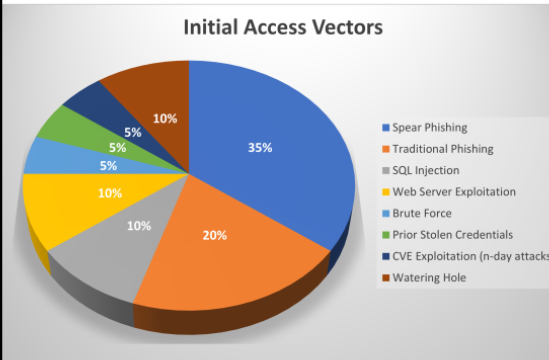
\includegraphics[width=1\textwidth]{initial-attack.png}
    \caption{初始入侵方法比例}
    \label{fig:fake_site}
\end{figure}

\subsection{APT與釣魚攻擊}
隨著數位化的迅速推進,企業和組織對網路安全的需求不斷增加。根據《PHISHING ACTIVITY TRENDS REPORT 4th Quarter 2023》,APWG 在2023年共觀察到4,987,809次釣魚攻擊,接近五百萬次,成為有記錄以來最嚴重的一年,超越2022年的4.7百萬次。這顯示釣魚攻擊的規模和頻率持續上升,攻擊手法也日益多樣化和精密化。\cite{apwg2023}

根據圖一我們可以發現,在高階持續性威脅(APT)攻擊中,網路釣魚經常作為首要攻擊步驟,其使用頻率超過了五成。攻擊者會夠過網路釣魚突破企業防線,深入系統內部。而釣魚攻擊作為 APT 的起點,通常依賴於社交工程技巧來騙取受害者的信任,讓他們主動點擊惡意連結或下載惡意軟體,這使得傳統的防禦機制難以有效偵測。


% 研究方法及步驟
\section{研究方法及步驟}
本學期之研究旨在模擬針對師大學生的釣魚攻擊情境,模擬目標為收集目標之帳號與密碼,並盡可能逼真地還原師大 Moodle 登錄介面(\url{https://moodle3.ntnu.edu.tw/login/index.php})。以下為研究的具體方法及實施步驟:

\begin{enumerate}

    \item \textbf{網頁介面模擬}:
     使用 Python 腳本爬取師大 Moodle 登錄介面的 HTML 與相關資源文件(如 CSS 和 JavaScript),以便生成一個初步的本地副本。完成後,前往 \href{https://fontawesome.com/}{Font Awesome}網站下載必要的 icon 資源,並對 HTML 文件進行手動編輯,確保外觀與功能與官方登錄頁面保持高度一致。
    
    \item \textbf{後端釣魚系統開發}:
    基於 Flask 後端技術,開發釣魚網頁的伺服端功能。被害人輸入的帳號與密碼將透過表單提交到後端伺服器,並儲存於一個安全的數據庫或文件中供後續分析。為降低被害人警惕性,後端邏輯會在接收到帳號與密碼後,自動將用戶重新導向至官方的師大 Moodle 登錄介面,模擬真實的登錄過程。
    
    \item \textbf{釣魚域名申請}:
    為進一步提升釣魚網站的真實性,我們註冊了一個與師大 Moodle 網站域名(\texttt{moodle3.ntnu.edu.tw})極為相似的 DNS:\texttt{ntnu.work.gd},並設置了別名 \texttt{moodle3.ntnu.work.gd}。此外,為避免瀏覽器顯示不安全的警告提示,我們為該域名配置了 HTTPS 憑證。釣魚網站還模擬了與官方登錄頁面一致的三個路徑,包括 \url{https://moodle3.ntnu.work.gd/}、\url{https://moodle3.ntnu.work.gd/login/} 和 \url{https://moodle3.ntnu.work.gd/login/index.php},進一步增強網站的欺騙性。
    
    \item \textbf{測試與改進}:
    在完成釣魚網站後,邀請部分志願者進行測試,模擬登錄行為並記錄釣魚網站的表現與穩定性,並對志願者進行訪問,以探討釣魚攻擊的有效性及後續改進方向。根據測試結果調整釣魚網站的設計,確保其穩定性、真實性與有效性。
    
\end{enumerate}


% 實驗結果
\section{實驗結果}
\url{https://moodle3.ntnu.work.gd/login/index.php} 是我們最終釣魚網站實作的成果,其效果如圖二至圖五所示。從圖中可以觀察到,除了 DNS 有些許差異外(官方網站的域名為 \texttt{.edu.tw},而我們的釣魚網站則為 \texttt{.work.gd)},釣魚網站的網頁 UI 幾乎與官方正版登錄界面完全一致,難以區分真偽,而在網頁互動功能上,釣魚網站則與官方網站毫無區別,綜合外觀與功能性,我們的釣魚網站具有以假亂真的能力。

\begin{figure}[ht!]
    \centering
    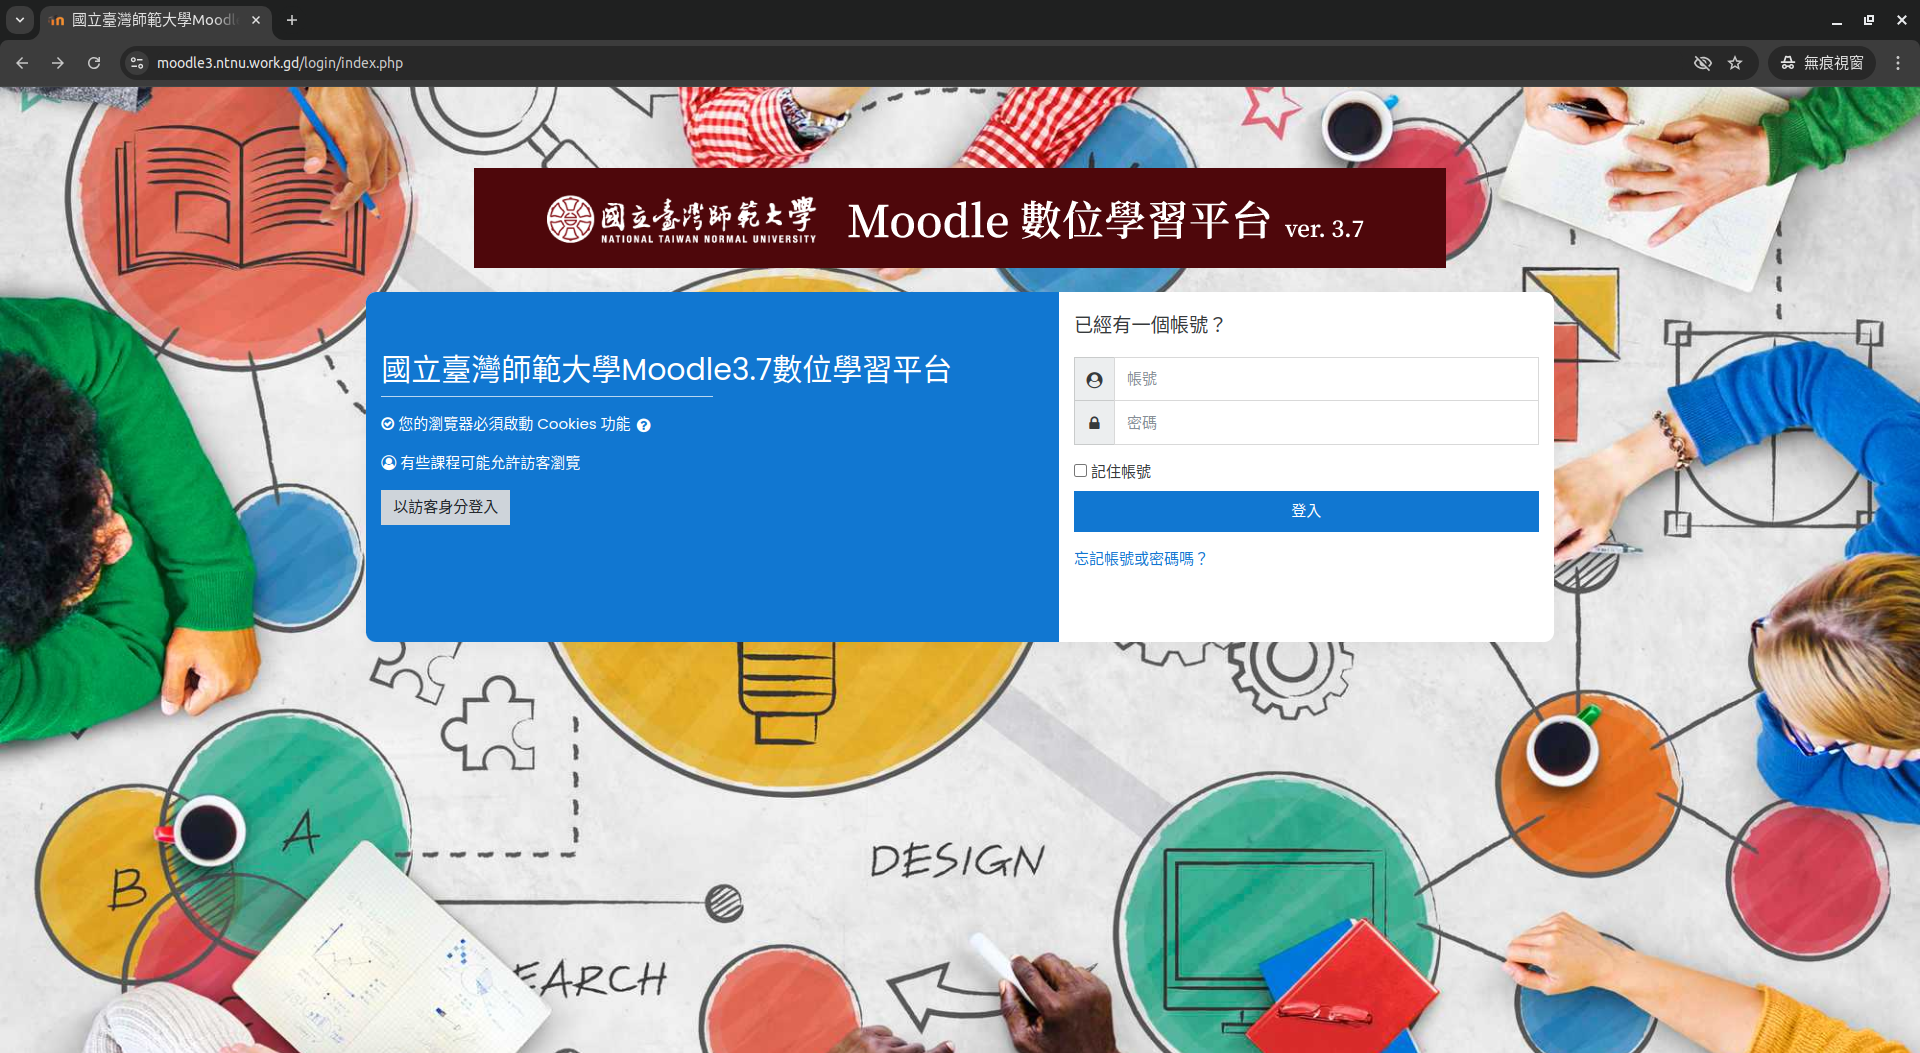
\includegraphics[width=1\textwidth]{pc_fake.png}
    \caption{電腦版的假 ntnu moodle}
    \label{fig:fake_site}
\end{figure}

\begin{figure}[ht!]
    \centering
    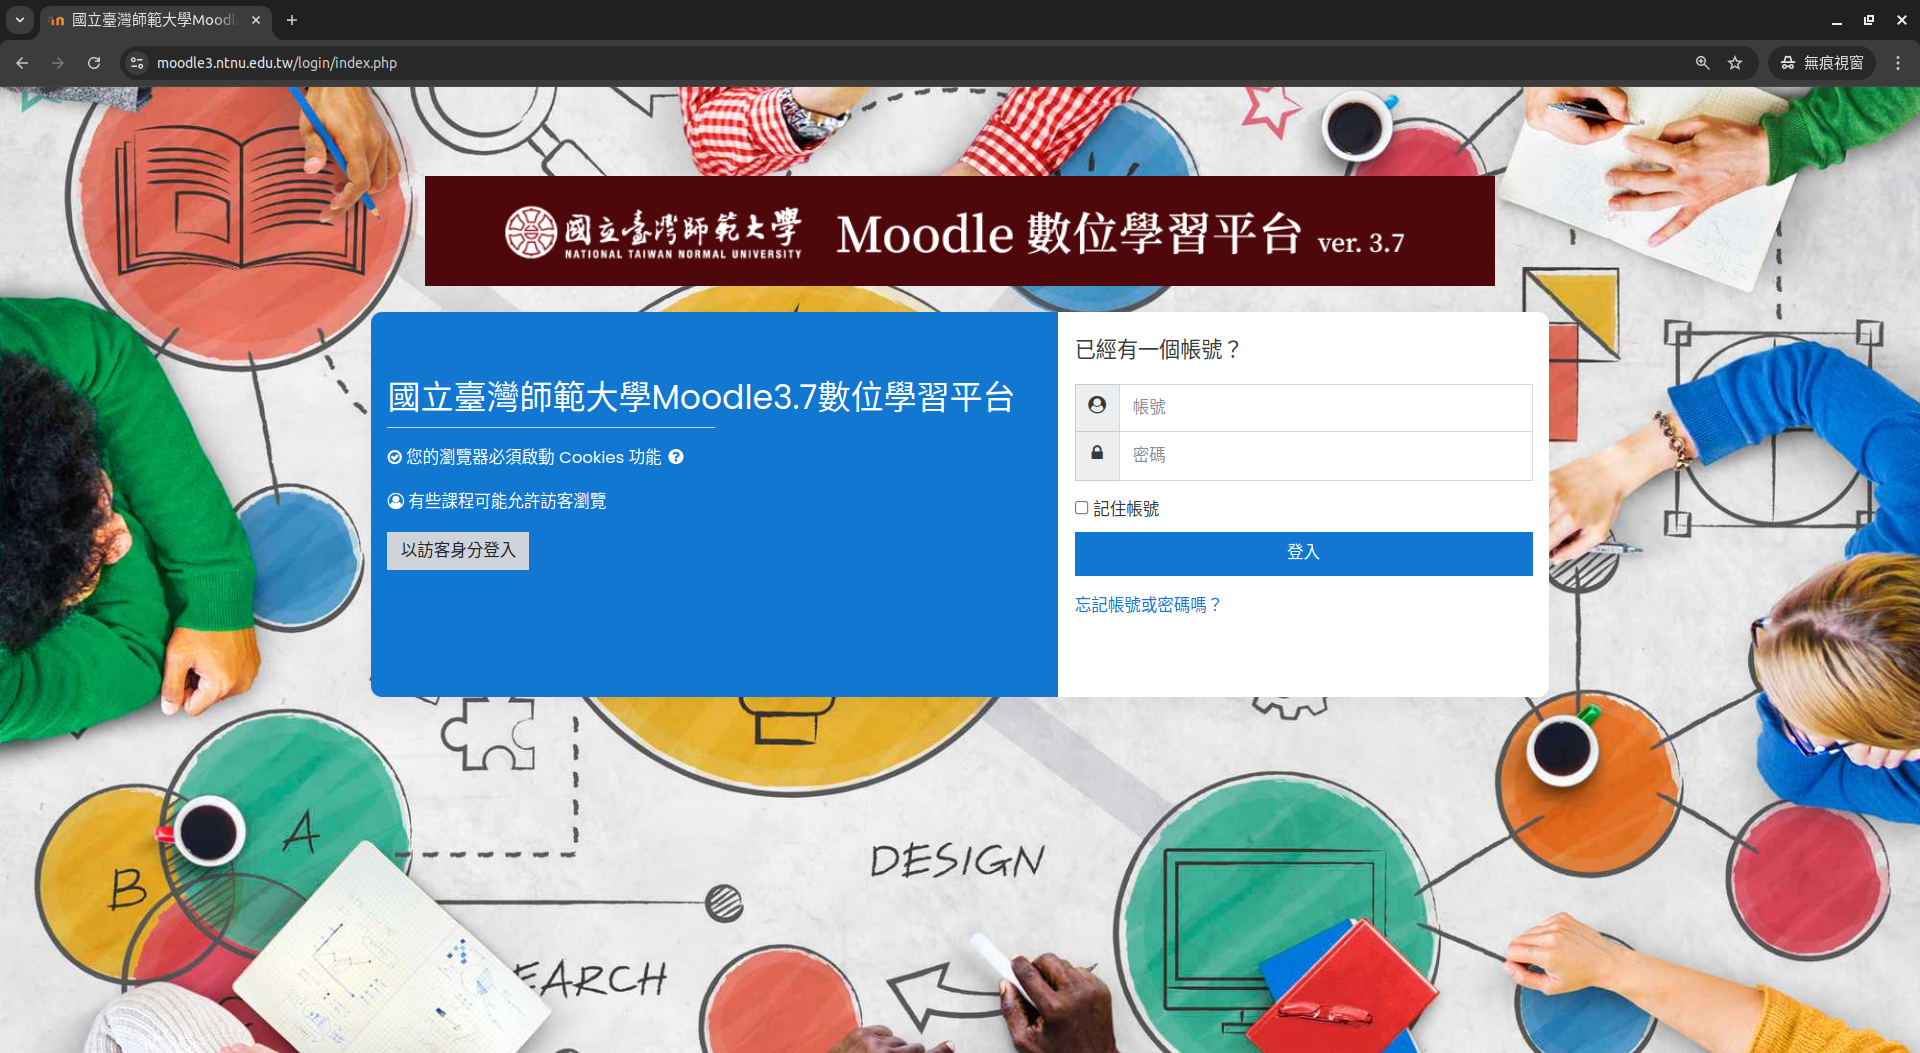
\includegraphics[width=1\textwidth]{pc_real.png}
    \caption{電腦版的真 ntnu moodle }
    \label{fig:real_site}
\end{figure}

\begin{figure}[ht!]
    \centering
    \begin{minipage}{0.45\textwidth}
        \centering
        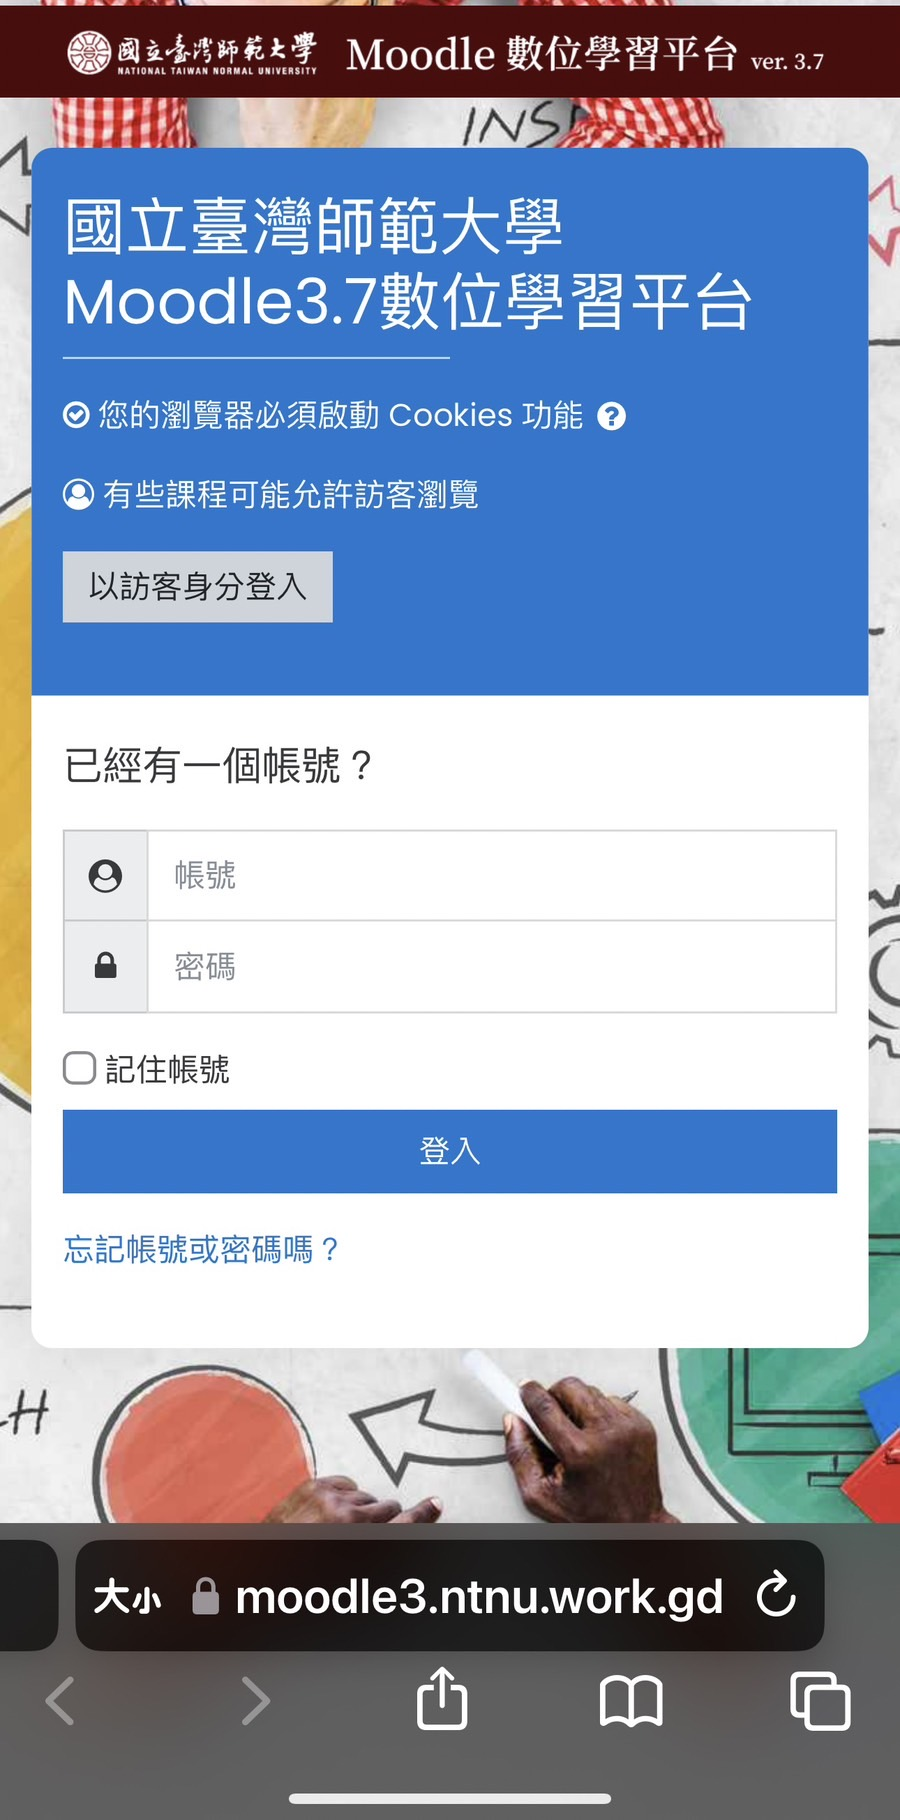
\includegraphics[width=\textwidth]{phone_fake.jpg}
        \caption{手機版的假 ntnu moodle}
        \label{fig:fake_site}
    \end{minipage}
    \hfill
    \begin{minipage}{0.45\textwidth}
        \centering
        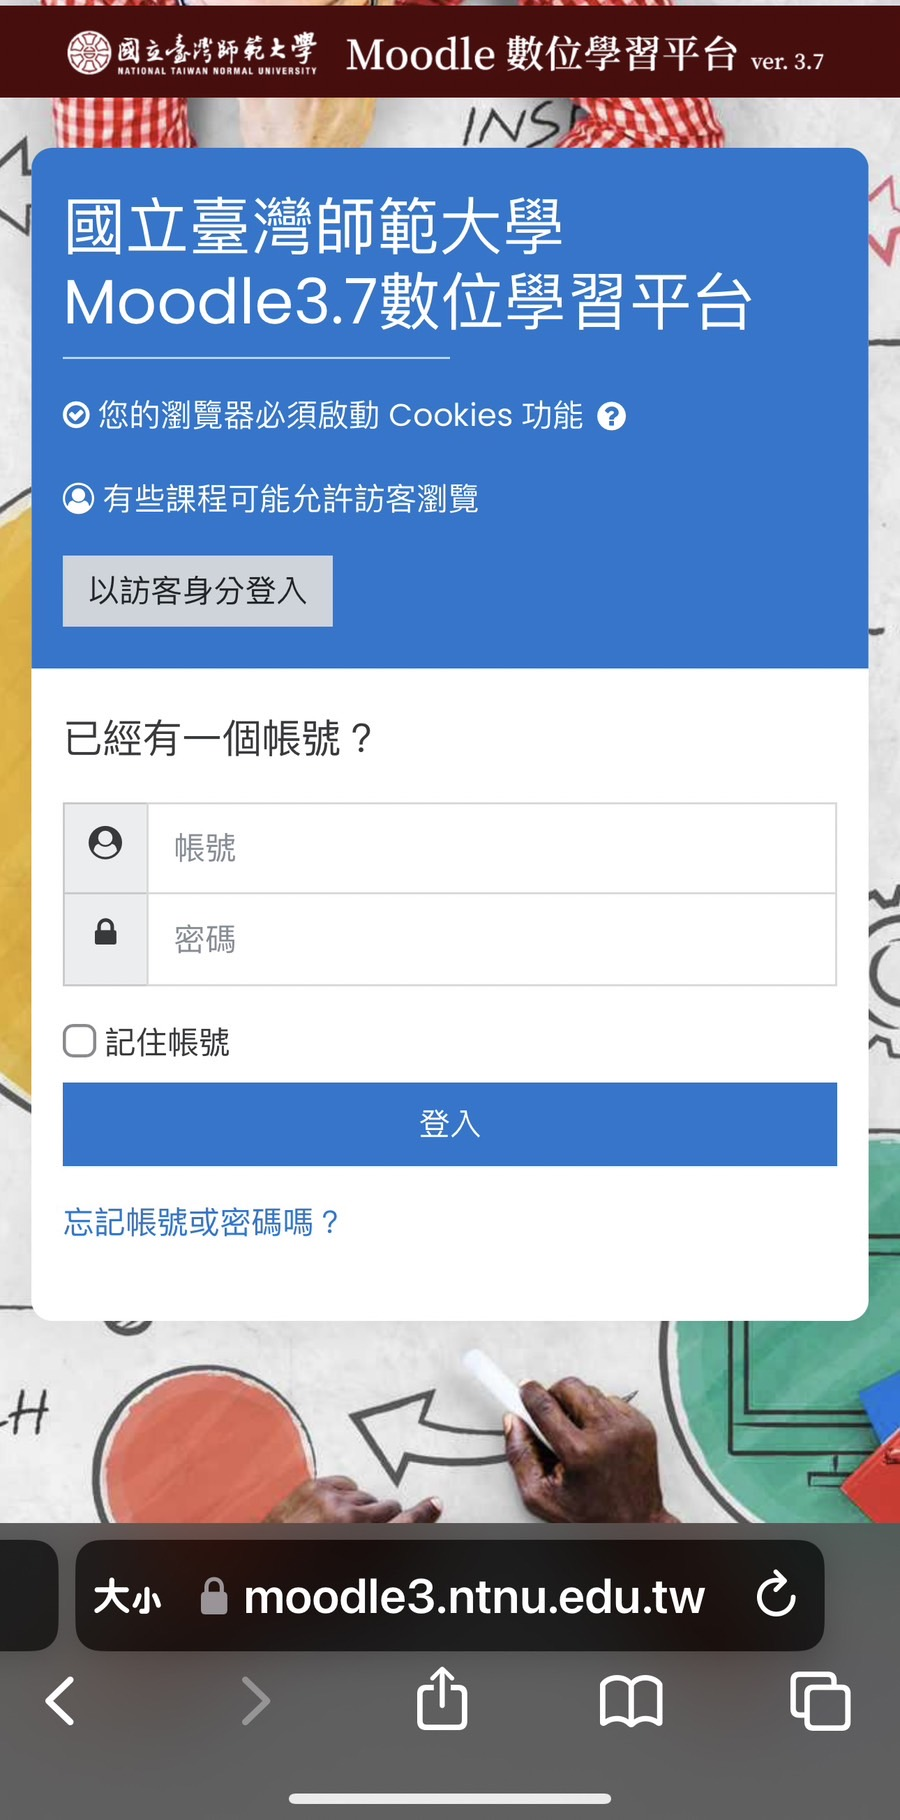
\includegraphics[width=\textwidth]{phone_real.jpg}
        \caption{手機版的真 ntnu moodle}
        \label{fig:real_site}
    \end{minipage}
\end{figure}


%分析與討論
\section{分析與討論}

本次實驗的結果顯示,釣魚網站與官方網站之間的相似度會大大地影響可信度,從而直接影響了攻擊的成功率。以下幾個關鍵點值得進一步探討:

\begin{enumerate}
	
    \item \textbf{DNS 混淆的有效性}:   
    使用類似於官方域名的自訂 DNS(如 \texttt{moodle3.ntnu.work.gd/login/index.php}),能有效降低受害者對網站真實性的懷疑。在模擬中,僅有高度警覺的用戶可能會通過觀察域名的細微差異察覺異常。
    
    \item \textbf{UI 的仿真效果}:  
    網頁 UI 的高度還原是本次實驗的另一大亮點。透過複製官方網站的 HTML、CSS 與 JavaScript,並進行手動調整,釣魚網站成功達到了與官方網站幾乎一致的視覺效果。這說明在針對非高度警覺的用戶時,這種仿真策略可以顯著提升攻擊成功率。
    
    \item \textbf{重定向策略的迷惑性}:  
    被害人在釣魚網站輸入帳號與密碼後,系統會自動將其導向至官方網站(\url{https://moodle3.ntnu.edu.tw/login/index.php}),進一步降低被害者的警覺性。這種策略能讓受害者誤以為其登錄過程正常,從而延遲發現攻擊的真相。
    
    \item \textbf{潛在防禦點的分析}:  
    本次模擬的成果揭示了防禦釣魚攻擊的幾個關鍵環節:
    \begin{enumerate}
    
        \item \textbf{域名檢查}:強調用戶在訪問網站時應注意 DNS 的完整性,並引導用戶識別 \texttt{.edu.tw} 等官方域名。
        \item \textbf{瀏覽器提示迷思}:許多人認為瀏覽器的 HTTPS 安全提示能有效提高用戶對釣魚網站的識別能力。然而,這實際上是一個迷思,因為駭客可以輕易地為釣魚網站申請並獲取合法的 SSL 憑證。由於免費且自動化的憑證服務(如 \texttt{Let's Encrypt})的普及,釣魚網站看似「安全」的 HTTPS 標誌可能進一步降低受害者的警覺性。因此,僅依賴 HTTPS 標誌作為判斷網站真偽的依據是遠遠不夠的。
        \item \textbf{用戶教育}:加強對用戶的釣魚攻擊防範意識教育,特別是針對常見的釣魚手段(如針對性釣魚郵件與模擬網站)。
        \item \textbf{防爬蟲機制}:官方網站應設置防爬蟲機制,以避免不肖人士輕易複製網頁 UI 來製作釣魚網站進行駭客攻擊。
    
    \end{enumerate}

\end{enumerate}

這些防禦點的分析揭示了現有防禦措施的不足之處,同時也指出了未來改進的方向。域名檢查和用戶教育是目前最為基礎但卻最有效的防禦手段,因為它們直接針對攻擊者利用的社交工程技巧。此外,澄清瀏覽器提示的迷思有助於用戶更理性地判斷網站的真偽,而防爬蟲機制則能夠從技術層面阻止釣魚網站的製作。


% 結論
\section{結論}
本研究探討了釣魚攻擊在高階持續性威脅(Advanced Persistent Threat, APT)中的應用,並通過實際製作釣魚網站模擬攻擊流程,驗證釣魚技術的有效性。首先,使用類似官方域名的自訂 DNS 有效降低了受害者對網站真實性的懷疑,顯著提升了釣魚網站的欺騙性。僅有少數高度警覺的用戶能夠通過細微的域名差異察覺異常,表明 DNS 混淆策略在實際攻擊中具有高效性。其次,釣魚網站的 UI 高度仿真顯著增加了攻擊的成功率。通過複製官方網站的 HTML、CSS 與 JavaScript,釣魚網站在視覺效果和功能性上幾乎與官方網站無異,這使得非高度警覺的用戶更容易上當受騙。此外,重定向策略的應用進一步迷惑了受害者。在用戶輸入帳號與密碼後,系統自動將其導向官方網站,延遲了受害者對釣魚攻擊的發現時間,從而增加了攻擊者獲取敏感信息的機會。最後,研究揭示了多個潛在的防禦點,包括加強域名檢查、澄清瀏覽器安全提示的迷思、提升用戶教育以及設置防爬蟲機制。這些防禦措施能夠在一定程度上減少釣魚攻擊的成功率,提升整體網路安全防護水平。

% 未來方向
\section{未來方向}
基於本研究的發現,未來的研究可以在以下幾個方面進行深入探討:

\begin{enumerate}

    \item \textbf{釣魚網站的 UI 改進與防禦策略設計}:
    本研究展示了釣魚網站在 UI 仿真方面的高效性,未來研究可以進一步探討如何改進釣魚網站的 UI 設計,以提高攻擊的成功率。同時,應研究如何利用 UI 設計本身來增強防禦,例如通過識別異常的 UI 元素或行為模式來及早偵測釣魚攻擊。

    \item \textbf{針對師大選課系統與校務行政系統的釣魚網站模擬研究}:
    本研究選擇了師大 Moodle 系統作為釣魚網站的模擬目標,未來可以擴展至師大其他關鍵系統,如選課系統與校務行政系統。通過模擬這些系統的釣魚攻擊,研究其特有的攻擊向量和防禦策略。此外,應分析不同系統的安全需求,並設計針對性的防禦措施,以提高這些關鍵系統的整體安全性。
    
    \item \textbf{現有釣魚攻擊辨別技術的研究與改進}:
    目前已有多種釣魚攻擊辨別技術,包括基於內容分析、URL 特徵分析以及機器學習方法等。然而,隨著攻擊技術的不斷演進,這些技術面臨著越來越多的挑戰。未來的研究應聚焦於評估現有技術的效能,並探索如何結合多種技術以提升辨別準確率。此外,應考慮引入深度學習等先進技術,以應對更為複雜和隱蔽的釣魚攻擊手法。

    \item \textbf{用戶行為與防禦意識研究}:
    深入研究不同用戶群體對釣魚攻擊的防範意識和行為反應,從而設計更具針對性的教育與培訓方案,提升整體用戶的安全意識。

    \item \textbf{多因素身份驗證的應用與效果評估}:
    探討多因素身份驗證(Multi-Factor Authentication, MFA)在防範釣魚攻擊中的應用效果,並評估其在實際運營環境中的可行性和用戶接受度。

\end{enumerate}

通過以上研究方向的深入探索,將有助於全面提升網路安全防護能力,減少釣魚攻擊帶來的風險。
% 參考文獻
%\section{參考文獻}
\begin{thebibliography}{9} % 數字 9 表示引用文獻的最大序號寬度

\bibitem{2014aptstudy} 
Ping Chen, Lieven Desmet, and Christophe Huygens, 
\textit{A Study on Advanced Persistent Threats}, 
Communications and Multimedia Security (CMS), Lecture Notes in Computer Science, vol. 8735, pp. 63--72, Springer, 2014.

\bibitem{iranianAPT} 
Ryan Simons, 
\textit{Investigating Initial Access Strategies and Malware Deployment Tactics Used by Iranian Advanced Persistent Threat Groups}, 
2023 IEEE International Conference on Big Data (BigData), IEEE, December 2023, Sorrento, Italy. 

\bibitem{apwg2023} 
APWG, \textit{PHISHING ACTIVITY TRENDS REPORT 4th Quarter 2023}, 
APWG, 2023. Available at: \url{https://docs.apwg.org/reports/apwg_trends_report_q4_2023.pdf}.


\end{thebibliography}


% 結束文件
\end{document}

